% Options for packages loaded elsewhere
\PassOptionsToPackage{unicode}{hyperref}
\PassOptionsToPackage{hyphens}{url}
\PassOptionsToPackage{dvipsnames,svgnames,x11names}{xcolor}
%
\documentclass[
  11pt,
  a4paper,
]{article}

\usepackage{amsmath,amssymb}
\usepackage{setspace}
\usepackage{iftex}
\ifPDFTeX
  \usepackage[T1]{fontenc}
  \usepackage[utf8]{inputenc}
  \usepackage{textcomp} % provide euro and other symbols
\else % if luatex or xetex
  \usepackage{unicode-math}
  \defaultfontfeatures{Scale=MatchLowercase}
  \defaultfontfeatures[\rmfamily]{Ligatures=TeX,Scale=1}
\fi
\usepackage{lmodern}
\ifPDFTeX\else  
    % xetex/luatex font selection
\fi
% Use upquote if available, for straight quotes in verbatim environments
\IfFileExists{upquote.sty}{\usepackage{upquote}}{}
\IfFileExists{microtype.sty}{% use microtype if available
  \usepackage[]{microtype}
  \UseMicrotypeSet[protrusion]{basicmath} % disable protrusion for tt fonts
}{}
\makeatletter
\@ifundefined{KOMAClassName}{% if non-KOMA class
  \IfFileExists{parskip.sty}{%
    \usepackage{parskip}
  }{% else
    \setlength{\parindent}{0pt}
    \setlength{\parskip}{6pt plus 2pt minus 1pt}}
}{% if KOMA class
  \KOMAoptions{parskip=half}}
\makeatother
\usepackage{xcolor}
\usepackage[top=2.4cm,bottom=2.4cm,left=2.5cm,right=2.5cm]{geometry}
\setlength{\emergencystretch}{3em} % prevent overfull lines
\setcounter{secnumdepth}{2}


\providecommand{\tightlist}{%
  \setlength{\itemsep}{0pt}\setlength{\parskip}{0pt}}\usepackage{longtable,booktabs,array}
\usepackage{calc} % for calculating minipage widths
% Correct order of tables after \paragraph or \subparagraph
\usepackage{etoolbox}
\makeatletter
\patchcmd\longtable{\par}{\if@noskipsec\mbox{}\fi\par}{}{}
\makeatother
% Allow footnotes in longtable head/foot
\IfFileExists{footnotehyper.sty}{\usepackage{footnotehyper}}{\usepackage{footnote}}
\makesavenoteenv{longtable}
\usepackage{graphicx}
\makeatletter
\newsavebox\pandoc@box
\newcommand*\pandocbounded[1]{% scales image to fit in text height/width
  \sbox\pandoc@box{#1}%
  \Gscale@div\@tempa{\textheight}{\dimexpr\ht\pandoc@box+\dp\pandoc@box\relax}%
  \Gscale@div\@tempb{\linewidth}{\wd\pandoc@box}%
  \ifdim\@tempb\p@<\@tempa\p@\let\@tempa\@tempb\fi% select the smaller of both
  \ifdim\@tempa\p@<\p@\scalebox{\@tempa}{\usebox\pandoc@box}%
  \else\usebox{\pandoc@box}%
  \fi%
}
% Set default figure placement to htbp
\def\fps@figure{htbp}
\makeatother

\makeatletter
\@ifpackageloaded{caption}{}{\usepackage{caption}}
\AtBeginDocument{%
\ifdefined\contentsname
  \renewcommand*\contentsname{Table of contents}
\else
  \newcommand\contentsname{Table of contents}
\fi
\ifdefined\listfigurename
  \renewcommand*\listfigurename{List of Figures}
\else
  \newcommand\listfigurename{List of Figures}
\fi
\ifdefined\listtablename
  \renewcommand*\listtablename{List of Tables}
\else
  \newcommand\listtablename{List of Tables}
\fi
\ifdefined\figurename
  \renewcommand*\figurename{Figure}
\else
  \newcommand\figurename{Figure}
\fi
\ifdefined\tablename
  \renewcommand*\tablename{Table}
\else
  \newcommand\tablename{Table}
\fi
}
\@ifpackageloaded{float}{}{\usepackage{float}}
\floatstyle{ruled}
\@ifundefined{c@chapter}{\newfloat{codelisting}{h}{lop}}{\newfloat{codelisting}{h}{lop}[chapter]}
\floatname{codelisting}{Listing}
\newcommand*\listoflistings{\listof{codelisting}{List of Listings}}
\makeatother
\makeatletter
\makeatother
\makeatletter
\@ifpackageloaded{caption}{}{\usepackage{caption}}
\@ifpackageloaded{subcaption}{}{\usepackage{subcaption}}
\makeatother

\usepackage[style=authoryear-comp,]{biblatex}
\usepackage{bookmark}

\IfFileExists{xurl.sty}{\usepackage{xurl}}{} % add URL line breaks if available
\urlstyle{same} % disable monospaced font for URLs
\hypersetup{
  pdftitle={Assignment 3 by team Ctrl+Alt+Analyze},
  pdfauthor={Malaika; Kunal; ZuxiLu},
  colorlinks=true,
  linkcolor={blue},
  filecolor={Maroon},
  citecolor={Blue},
  urlcolor={Blue},
  pdfcreator={LaTeX via pandoc}}

%% CAPTIONS
\usepackage{caption}
\DeclareCaptionStyle{italic}[justification=centering]
 {labelfont={bf},textfont={it},labelsep=colon}
\captionsetup[figure]{style=italic,format=hang,singlelinecheck=true}
\captionsetup[table]{style=italic,format=hang,singlelinecheck=true}

%% FONT
\usepackage{bera}
\usepackage[charter]{mathdesign}
\usepackage[scale=0.9]{sourcecodepro}
\usepackage[lf,t]{FiraSans}
\usepackage{fontawesome}

%% HEADERS AND FOOTERS
\usepackage{fancyhdr}
\pagestyle{fancy}
\rfoot{\Large\sffamily\raisebox{-0.1cm}{\textbf{\thepage}}}
\makeatletter
\lhead{\textsf{\expandafter{\@title}}}
\makeatother
\rhead{}
\cfoot{}
\setlength{\headheight}{15pt}
\renewcommand{\headrulewidth}{0.4pt}
\renewcommand{\footrulewidth}{0.4pt}
\fancypagestyle{plain}{%
\fancyhf{} % clear all header and footer fields
\fancyfoot[C]{\sffamily\thepage} % except the center
\renewcommand{\headrulewidth}{0pt}
\renewcommand{\footrulewidth}{0pt}}

%% MATHS
\usepackage{bm,amsmath}
\allowdisplaybreaks

%% GRAPHICS
\makeatletter
\def\fps@figure{htbp}
\makeatother
\setcounter{topnumber}{2}
\setcounter{bottomnumber}{2}
\setcounter{totalnumber}{4}
\renewcommand{\topfraction}{0.85}
\renewcommand{\bottomfraction}{0.85}
\renewcommand{\textfraction}{0.15}
\renewcommand{\floatpagefraction}{0.8}

%% SECTION TITLES
\usepackage[compact,sf,bf]{titlesec}
\titleformat*{\section}{\Large\sf\bfseries\color[rgb]{0.7,0,0}}
\titleformat*{\subsection}{\large\sf\bfseries\color[rgb]{0.7,0,0}}
\titleformat*{\subsubsection}{\sf\bfseries\color[rgb]{0.7,0,0}}
\titlespacing{\section}{0pt}{*5}{*1}
\titlespacing{\subsection}{0pt}{*2}{*0.2}
\titlespacing{\subsubsection}{0pt}{*1}{*0.1}

%% BIBLIOGRAPHY.

\makeatletter
\@ifpackageloaded{biblatex}{
\ExecuteBibliographyOptions{bibencoding=utf8,minnames=1,maxnames=3, maxbibnames=99,dashed=false,terseinits=true,giveninits=true,uniquename=false,uniquelist=false,doi=false, isbn=false,url=true,sortcites=false}
\DeclareFieldFormat{url}{\texttt{\url{#1}}}
\DeclareFieldFormat[article]{pages}{#1}
\DeclareFieldFormat[inproceedings]{pages}{\lowercase{pp.}#1}
\DeclareFieldFormat[incollection]{pages}{\lowercase{pp.}#1}
\DeclareFieldFormat[article]{volume}{\mkbibbold{#1}}
\DeclareFieldFormat[article]{number}{\mkbibparens{#1}}
\DeclareFieldFormat[article]{title}{\MakeCapital{#1}}
\DeclareFieldFormat[article]{url}{}
\DeclareFieldFormat[inproceedings]{title}{#1}
\DeclareFieldFormat{shorthandwidth}{#1}
\usepackage{xpatch}
\xpatchbibmacro{volume+number+eid}{\setunit*{\adddot}}{}{}{}
% Remove In: for an article.
\renewbibmacro{in:}{%
  \ifentrytype{article}{}{%
  \printtext{\bibstring{in}\intitlepunct}}}
\AtEveryBibitem{\clearfield{month}}
\AtEveryCitekey{\clearfield{month}}
\DeclareDelimFormat[cbx@textcite]{nameyeardelim}{\addspace}
\renewcommand*{\finalnamedelim}{\addspace\&\space}
}{}
\makeatother

%% PAGE BREAKING to avoid widows and orphans
\clubpenalty = 2000
\widowpenalty = 2000
\usepackage{microtype}
% Placement of logos

\RequirePackage[absolute,overlay]{textpos}
\setlength{\TPHorizModule}{1cm}
\setlength{\TPVertModule}{1cm}
\def\placefig#1#2#3#4{\begin{textblock}{.1}(#1,#2)\rlap{\includegraphics[#3]{#4}}\end{textblock}}

% Title and date

\title{Assignment 3 by team Ctrl+Alt+Analyze}
\date{30 May 2025}

\def\Date{\number\day}
\def\Month{\ifcase\month\or
 January\or February\or March\or April\or May\or June\or
 July\or August\or September\or October\or November\or December\fi}
\def\Year{\number\year}

%%%% PAGE STYLE FOR FRONT PAGE OF REPORTS

\makeatletter
\def\organization#1{\gdef\@organization{#1}}
\def\telephone#1{\gdef\@telephone{#1}}
\def\email#1{\gdef\@email{#1}}
\makeatother
  \organization{}

  \def\name{Department of\newline Econometrics \&\newline Business Statistics}

  \telephone{(03) 9903 4416}

  \email{BusEco-Econometrics@monash.edu}

\def\webaddress{\url{https://www.monash.edu/business/ebs}}
\def\abn{12 377 614 012}
\def\extraspace{\vspace*{1.6cm}}
\makeatletter
\def\contactdetails{\faicon{phone} & \@telephone \\
                    \faicon{envelope} & \@email}
\makeatother

\usepackage[absolute,overlay]{textpos}
\setlength{\TPHorizModule}{1cm}
\setlength{\TPVertModule}{1cm}

%%%% FRONT PAGE OF REPORTS

\def\reporttype{Report for}

\long\def\front#1#2#3{
\newpage
\begin{textblock}{7}(12.7,28.2)\hfill

\includegraphics[height=0.6cm]{AACSB}~~~

\includegraphics[height=0.6cm]{EQUIS}~~~

\includegraphics[height=0.6cm]{AMBA}
\end{textblock}
\begin{singlespacing}
\thispagestyle{empty}
\vspace*{-1.4cm}
\hspace*{-1.4cm}
\hbox to 16cm{
  \hbox to 6.5cm{\vbox to 14cm{\vbox to 25cm{
    
\includegraphics[width=6cm]{monash2}
    \vfill
    
\includegraphics[width=2cm]{MBSportrait}
    \vspace{0.4cm}
    \par
    \parbox{6.3cm}{\raggedright
      \sf\color[rgb]{0.00,0.00,0.70}
      {\large\textbf{\name}}\par
      \vspace{.7cm}
      \tabcolsep=0.12cm\sf\small
      \begin{tabular}{@{}ll@{}}\contactdetails
      \end{tabular}
      \vspace*{0.3cm}\par
      ABN: \abn\par
    }
  }\vss}\hss}
  \hspace*{0.2cm}
  \hbox to 1cm{\vbox to 14cm{\rule{1pt}{26.8cm}\vss}\hss\hfill}
  \hbox to 10cm{\vbox to 14cm{\vbox to 25cm{
      \vspace*{3cm}\sf\raggedright
      \parbox{10cm}{\sf\raggedright\baselineskip=1.2cm
         \fontsize{24.88}{30}\color[rgb]{0.70,0.00,0.00}\sf\textbf{#1}}
      \par
      \vfill
      \large
      \vbox{\parskip=0.8cm #2}\par
      \vspace*{2cm}\par
      \reporttype\\[0.3cm]
      \hbox{#3}%\\[2cm]\
      \vspace*{1cm}
      {\large\sf\textbf{\Date~\Month~\Year}}
   }\vss}
  }}
\end{singlespacing}
\newpage
}

\makeatletter
\def\maketitle{\front{\expandafter{\@title}}{\@author}{\@organization}}
\makeatother

% Authors

\author{\sf{\Large\textbf{Malaika} \\[0.5cm]}{\Large\textbf{Kunal} \\[0.5cm]}{\Large\textbf{ZuxiLu} \\[0.5cm]}}
\lfoot{\sf Malaika, Kunal, ZuxiLu: 30 May 2025}
\begin{document}
\maketitle

\renewcommand*\contentsname{Table of contents}
{
\hypersetup{linkcolor=}
\setcounter{tocdepth}{3}
\tableofcontents
}

\setstretch{1.5}
\newpage

\section{Investigating the relationship between student's academic
performance and lifestyle
habits}\label{investigating-the-relationship-between-students-academic-performance-and-lifestyle-habits}

By Team : \textbf{Ctrl+Alt+Analyze}

Authors:

\begin{enumerate}
\def\labelenumi{\arabic{enumi}.}
\item
  \textbf{Malaika}
\item
  \textbf{Zuxilu}
\item
  \textbf{Kunal}
\end{enumerate}

\section{Executive summary}\label{executive-summary}

\begin{itemize}
\tightlist
\item
  This report investigates the relationship between student lifestyle
  habits and academic performance using correlation analysis. We
  classify study hours, class attendance, and sleep duration as ``good''
  habits, while the time spent on social media, and Netflix usage are
  treated as ``bad'' habits.
\item
  Our findings indicate that study hours have the strongest positive
  correlation with exam scores, while time spent on social media and
  Netflix show weak negative correlations. Results from our study can be
  used to guide and inform students about the relationship between their
  lifestyle choices and academic success.
\end{itemize}

\section{Introduction}\label{introduction}

Academic performance is influenced by a range of behavioral and
lifestyle factors. Habits such as consistent study routines, classroom
attendance, and adequate sleep are commonly associated with better exam
outcomes. In contrast, excessive time spent on social media and
streaming platforms may reduce focus and study time. This study aims to
quantify the relationship between these habits and academic performance
using correlation analysis. The dataset includes student-reported habits
and their corresponding exam scores. We define ``good habits'' as study
hours, class attendance, and sleep hours, and ``bad habits'' as social
media and Netflix usage. Using correlation matrices and visualizations,
we examine how each habit is associated with exam performance. Our goal
is to identify which habits have the strongest relationship with scores
and whether they are positive or negative. The findings may provide
insight into which behaviors support or hinder academic success. This
report is structured to include our methodology, results, discussion,
and recommendations.

\newpage

\section{Methodology}\label{methodology}

\begin{longtable}[]{@{}
  >{\raggedright\arraybackslash}p{(\linewidth - 8\tabcolsep) * \real{0.2529}}
  >{\raggedleft\arraybackslash}p{(\linewidth - 8\tabcolsep) * \real{0.2299}}
  >{\raggedleft\arraybackslash}p{(\linewidth - 8\tabcolsep) * \real{0.2529}}
  >{\raggedleft\arraybackslash}p{(\linewidth - 8\tabcolsep) * \real{0.1379}}
  >{\raggedleft\arraybackslash}p{(\linewidth - 8\tabcolsep) * \real{0.1264}}@{}}
\caption{Correlation matrix of good habits and exam
score}\tabularnewline
\toprule\noalign{}
\begin{minipage}[b]{\linewidth}\raggedright
\end{minipage} & \begin{minipage}[b]{\linewidth}\raggedleft
study\_hours\_per\_day
\end{minipage} & \begin{minipage}[b]{\linewidth}\raggedleft
attendance\_percentage
\end{minipage} & \begin{minipage}[b]{\linewidth}\raggedleft
sleep\_hours
\end{minipage} & \begin{minipage}[b]{\linewidth}\raggedleft
exam\_score
\end{minipage} \\
\midrule\noalign{}
\endfirsthead
\toprule\noalign{}
\begin{minipage}[b]{\linewidth}\raggedright
\end{minipage} & \begin{minipage}[b]{\linewidth}\raggedleft
study\_hours\_per\_day
\end{minipage} & \begin{minipage}[b]{\linewidth}\raggedleft
attendance\_percentage
\end{minipage} & \begin{minipage}[b]{\linewidth}\raggedleft
sleep\_hours
\end{minipage} & \begin{minipage}[b]{\linewidth}\raggedleft
exam\_score
\end{minipage} \\
\midrule\noalign{}
\endhead
\bottomrule\noalign{}
\endlastfoot
study\_hours\_per\_day & 1.00 & 0.03 & -0.03 & 0.83 \\
attendance\_percentage & 0.03 & 1.00 & 0.01 & 0.09 \\
sleep\_hours & -0.03 & 0.01 & 1.00 & 0.12 \\
exam\_score & 0.83 & 0.09 & 0.12 & 1.00 \\
\end{longtable}

This study used correlation analysis to explore the relationship between
student habits and academic performance. The dataset included 100
student records with variables such as study hours, class attendance,
sleep duration, social media usage, Netflix hours, and final exam
scores.

We categorized the variables into two groups:

\begin{itemize}
\item
  \textbf{Good habits:} StudyHours, AttendanceRate, SleepHours
\item
  \textbf{Bad habits:} SocialMediaHours, NetflixHours
\end{itemize}

Our target variable for academic performance was ExamScore. To analyze
relationships, we calculated Pearson correlation coefficients between
each habit variable and ExamScore. This approach allowed us to assess
the strength and direction of the linear relationship between variables.

Before analysis, variables were renamed for clarity (e.g.,
study\_hours\_per\_day → StudyHours). Only complete cases were used to
ensure accuracy. A correlation matrix was computed using cor() in R, and
visualized using \textbf{color-coded bar plots} to enhance
interpretability. Each bar displays the strength and direction of
correlation between a habit and exam performance. We also introduced an
Impact label that classifies habits as either \textbf{``Helps''} or
\textbf{``Hurts''} academic outcomes, based on whether their correlation
with exam scores is positive or negative.

\newpage

Figure 1 shows a bar plot of how good and bad habits correlate with exam
scores. Bars are color-coded to indicate positive (``Helps'') or
negative (``Hurts'') impact.

\pandocbounded{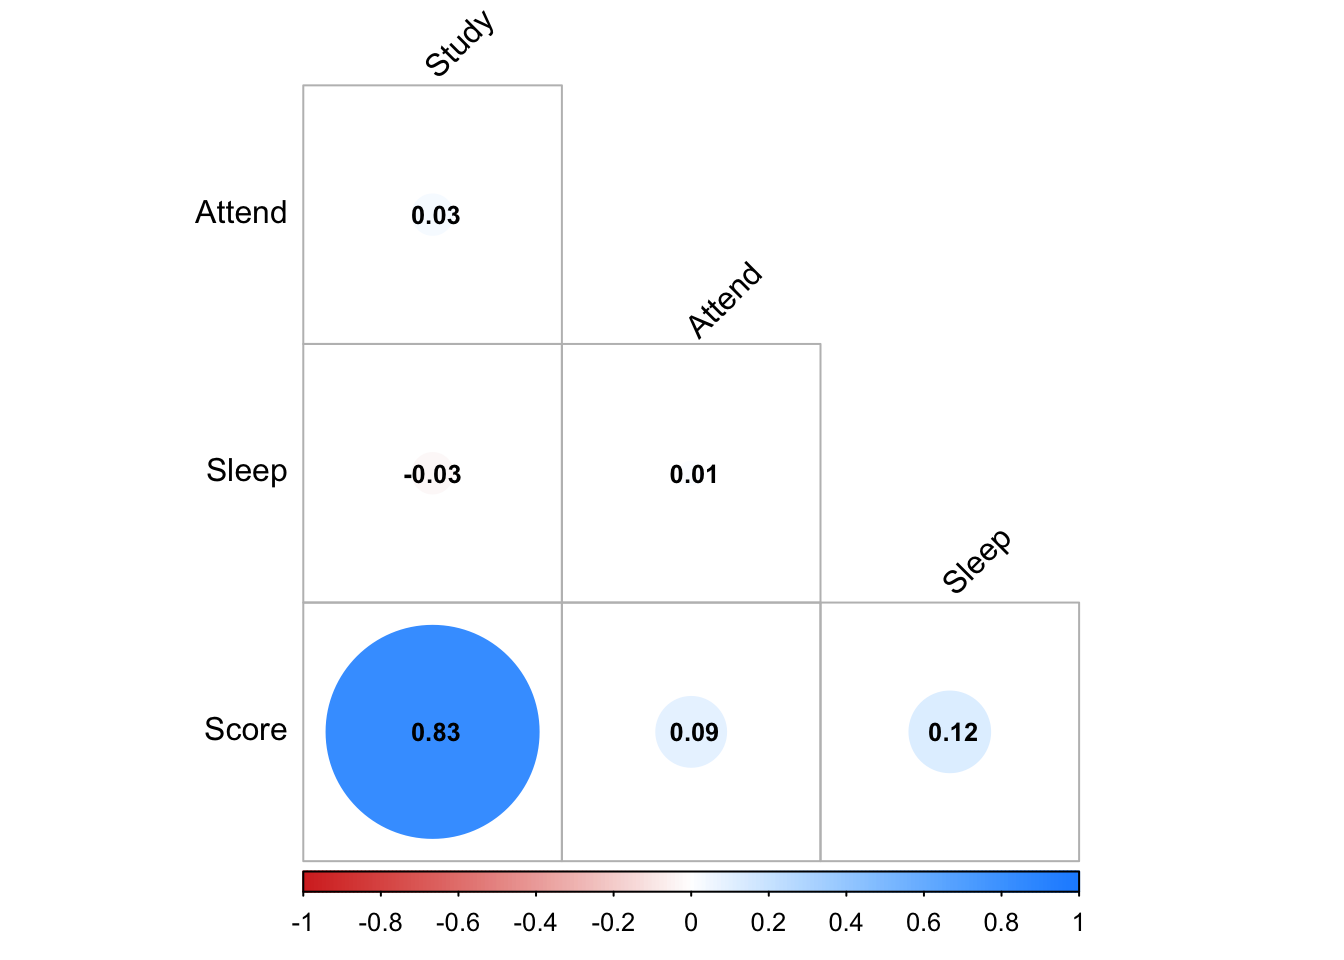
\includegraphics[keepaspectratio]{students-performance-analysis_files/figure-pdf/unnamed-chunk-5-1.pdf}}

\newpage

\section{Investigating `good' habits'}\label{investigating-good-habits}

\begin{itemize}
\item
  Figure 2 summarizes how StudyHours, AttendanceRate, and SleepHours
  relate to exam scores using a labeled bar plot.
\item
  \textbf{StudyHours} has a \textbf{strong positive correlation} with
  ExamScore (r = 0.83).

  \begin{itemize}
  \tightlist
  \item
    Students who study more tend to score higher.
  \end{itemize}
\item
  \textbf{AttendanceRate} and \textbf{SleepHours} both show \textbf{weak
  positive correlations}

  \begin{itemize}
  \tightlist
  \item
    Attendance (r = 0.09) and Sleep (r = 0.12) have little impact on
    scores.
  \end{itemize}
\item
  \textbf{Conclusion:} Among the good habits, \textbf{studying
  regularly} is clearly the most effective for better academic
  performance.
\item
  use Figure~\ref{fig-correlation-bar-plot}
\end{itemize}

\begin{figure}

\centering{

\pandocbounded{\includegraphics[keepaspectratio]{students-performance-analysis_files/figure-pdf/fig-correlation-bar-plot-1.pdf}}

}

\caption{\label{fig-correlation-bar-plot}How Habits Correlate with Exam
Performance}

\end{figure}%

\newpage

\section{Investigating `bad' habits'}\label{investigating-bad-habits}

\begin{itemize}
\item
  The chart shows how two bad habits relate to exam performance:

  \begin{itemize}
  \tightlist
  \item
    SocialMediaHours and NetflixHours.
  \end{itemize}
\item
  Both habits have \textbf{weak negative correlations} with ExamScore (r
  = -0.17 each).

  \begin{itemize}
  \tightlist
  \item
    More time spent on these may slightly lower scores.
  \end{itemize}
\item
  The two habits are \textbf{not correlated with each other} (r = 0.01).

  \begin{itemize}
  \tightlist
  \item
    Social media and Netflix usage appear to be independent.
  \end{itemize}
\item
  \textbf{Conclusion:} These habits may slightly harm performance, but
  the effect is \textbf{not strong} or highly predictive.
\end{itemize}

\begin{figure}

\centering{

\pandocbounded{\includegraphics[keepaspectratio]{students-performance-analysis_files/figure-pdf/fig-bad-habits-barplot-1.pdf}}

}

\caption{\label{fig-bad-habits-barplot}How Bad Habits Correlate with
Exam Performance}

\end{figure}%

\newpage

\section{Results:}\label{results}

The bar plots and Table~\ref{tbl-good-habits-correlation} summarize how
each lifestyle habit correlates with academic performance. The colors in
the plots indicate whether a habit \emph{helps} (positive correlation)
or \emph{hurts} (negative correlation) exam scores.

StudyHours shows the strongest positive relationship with ExamScore (r =
0.83), reinforcing its importance for academic success. AttendanceRate
(r = 0.09) and SleepHours (r = 0.12) show minor positive associations.

On the other hand, both SocialMediaHours and NetflixHours have weak
negative correlations with ExamScore (r = -0.17 each), suggesting these
habits may slightly hinder performance.

These patterns are visualized clearly through labeled bar plots, making
it easier to interpret the influence of each habit on academic
performance.

\begin{longtable}[]{@{}lr@{}}

\caption{\label{tbl-good-habits-correlation}Correlation with Exam Score
for Each Habit}

\tabularnewline

\toprule\noalign{}
& Correlation with ExamScore \\
\midrule\noalign{}
\endhead
\bottomrule\noalign{}
\endlastfoot
StudyHours & 0.83 \\
AttendanceRate & 0.09 \\
SleepHours & 0.12 \\
SocialMediaHours & -0.17 \\
NetflixHours & -0.17 \\

\end{longtable}

\newpage

\section{Discussion, Conclusion and
Recommendations:}\label{discussion-conclusion-and-recommendations}

\begin{itemize}
\item
  The findings from this analysis reinforce a key academic insight:
  consistent study habits have the strongest influence on student
  performance. Among all habits examined, StudyHours had the clearest
  and most substantial correlation with ExamScore (r = 0.83).
\item
  The updated bar plots simplify interpretation by highlighting which
  habits help or hurt academic performance. Habits like AttendanceRate
  and SleepHours offered minor positive impacts, while SocialMediaHours
  and NetflixHours showed weak negative correlations.
\item
  Introducing the ``Impact'' category (Helps/Hurts) made these trends
  easier to communicate visually, improving accessibility for all
  readers. While digital distractions like social media and Netflix
  usage may slightly reduce exam performance, they are not as
  significant as maintaining regular study routines.
\item
  Practically, students should focus on strengthening study habits while
  being mindful of time spent on digital entertainment. These
  recommendations are supported by clear visual evidence and measurable
  correlations.
\item
  Future studies could explore whether these relationships hold in
  larger or more diverse samples, or how other variables such as
  motivation or time management interact with these habits.
\end{itemize}

\section{References}\label{references}

\begin{enumerate}
\def\labelenumi{\arabic{enumi}.}
\item
  Dataset: Student Habits and Performance. Simulated dataset for
  academic use, 2025.
\item
  Ian, A., Syam, M. A., \& Rante, A. (2025). The Relationship Between
  Study Hours and Students' Academic Achievement. \emph{SSRN}.
  \url{https://ssrn.com/abstract=5124254}
\item
  Abbas, J., Aman, J., Nurunnabi, M., \& Bano, S. (2023). Association
  between social media use and students' academic performance: A
  structural equation modeling approach. \emph{Education and Information
  Technologies}, 28, 123--145.
  \url{https://link.springer.com/article/10.1007/s10639-023-12407-y}
\end{enumerate}


\printbibliography



\end{document}
